\documentclass[a5paper,12pt,twoside]{book}

\usepackage[tmargin=20mm,bmargin=25mm,lmargin=20mm,rmargin=20mm]{geometry} % Formato de página

\usepackage[output-decimal-marker={,}]{siunitx} % Unidades del SI
    \sisetup{per-mode = fraction}
    \DeclareSIUnit{\rpm}{rpm}
    \DeclareSIUnit{\atmosphere}{atm}

\usepackage[framemethod=TikZ]{mdframed} % Define \begin{mdframed}[style=MyFrame1]

    \mdfdefinestyle{MyFrame1}
    {linecolor=black!80!gray,
    outerlinewidth=0.5pt,
    roundcorner=0pt,
    innertopmargin=15pt,
    innerbottommargin=20pt,
    innerrightmargin=15pt,
    innerleftmargin=15pt,
    backgroundcolor=gray!30!white}

    \mdfdefinestyle{MyFrame2}
    {linecolor=white,
    outerlinewidth=0.5pt,
    roundcorner=10pt,
    innertopmargin=15pt,
    innerbottommargin=20pt,
    innerrightmargin=15pt,
    innerleftmargin=15pt,
    backgroundcolor=gray!20!white}

\usepackage{graphicx}
    \graphicspath{{./images/}} % Define \graphicspath{{dir1}{dir2}} para incluir imágenes que estén en los directorios dir1 y dir2

\usepackage[spanish]{babel}  % Traducciones y abreviaturas
\usepackage{amssymb}  % Símbolos y tipografía matemáticos
\usepackage{amsmath}  % Formato y estructura matemáticos
\usepackage{esint} % Define \oiint para integrales cerradas y acomoda \iiint
\usepackage{hyperref}  % Referencias cruzadas
\usepackage{fancyhdr}  % Encabezado y pie
\usepackage{graphicx}  % Define \includegraphics
\usepackage{pdfpages} % Define \includepdf
\usepackage{multicol} % Entorno de formato en columnas
\usepackage{comment} % Comenta todo entre \begin{comment} \end{comment}
% COMANDOS DE FORMATO
\newcommand{\sub}[2]{{{#1}_\textsl{{#2}}}} % #1 subíndice #2 (Usado cuando #2 es $texto$)
\newcommand{\scale}[2]{\text{\scalebox{#1}{$#2$}}} % Aplicar factor de escala #1 a la ecuación #2
\newcommand{\cusTi}[1]{\noindent\textbf{#1}} % Título de definiciones, propiedades y ejemplos
\newcommand{\cusTe}[1]{\vspace{2mm}\\\text{\hspace{\the\parindent}}#1} % Descripción de definiciones, propiedades y ejemplos
\newcommand{\noTi}[1]{\text{\hspace{\the\parindent}}#1} % Descripción de MyFrame1 que no tenga título
\newcommand{\concept}[1]{\vspace{1ex} \textsc{#1}} % Subtítulos sin jerarquía
\newcommand{\braces}[1]{{ \left\{ {#1} \right\} }} % #1 entre llaves
\newcommand{\sqb}[1]{{ \begin{bmatrix} #1 \end{bmatrix} }} % #1 entre corchetes
\newcommand{\bb}[1]{\left(#1\right)} % #1 entre paréntesis
\newcommand{\sfrac}[2]{#1/#2} % Fracciones #1/#2 para reemplazar el (muy lento) \usepackage{xfrac}
\newcommand{\captionSpace}{-0.8cm} % Espacio entre figuras y pie de foto

% COMANDOS PARA NOTACIÓN DE FUNCIONES
\newcommand{\barrow}[3]{\begin{bmatrix} \left. #1 \right|_{#2}^{#3} \end{bmatrix}} % Regla de Barrow de #1 para los extremos de integración #2 y #3
\newcommand{\fx}[2][f]{#1 \hspace{-0.5mm} \left( #2 \right)} % #1 en función de #2 con paréntesis
\newcommand{\ffx}[2][f]{#1 \hspace{-0.5mm} \begin{bmatrix} #2 \end{bmatrix}} % #1 en función de #2 con corchetes
\newcommand{\intProd}[2]{<\hspace{-0.8mm}#1,#2\hspace{-0.8mm}>} % Producto interno entre #1 y #2
\newcommand{\comb}[2]{\begin{pmatrix} {#1}\\{#2} \end{pmatrix}} % Combinatorio n=#1, m=#2
\newcommand{\media}[2]{\underset{#2}{\sub{#1}{med}}} % #1 media entre #2
\newcommand{\norm}[1]{{\left| {#1} \right|}} % Módulo de #1
\newcommand{\nnorm}[1]{{\left|\left| {#1} \right|\right|}} % Norma de #1
\newcommand{\trans}[1]{#1^*} % Matriz transpuesta de #1
\newcommand{\conj}[1]{\overline{#1}} % Conjugado de #1
\newcommand{\ave}[1]{\bar{#1}} % Valor promedio de #1
\newcommand{\rms}[1]{{\sub{#1}{ef}}} % Valor eficaz de #1
\newcommand{\peak}[1]{{\sub{#1}{pk}}} % Valor pico de #1

% COMANDOS PARA NOTACIÓN DE ELEMENTOS Y OPERADORES
\newcommand{\class}[1][1]{\mathcal{C}^{#1}} % Clase o cantidad de derivadas parciales contínuas
\newcommand{\versor}[1]{\hat{#1}} % Vector unitario #1
\newcommand{\fasor}[1]{\check{#1}} % Fasor #1
\newcommand{\iVer}{\versor{\imath}} % i versor
\newcommand{\jVer}{\versor{\jmath}} % j versor
\newcommand{\kVer}{\versor{k}} % k versor
\newcommand{\eVer}{\versor{\textbf{e}}} % Versor canónico
\newcommand{\tang}{\textbf{t}} % Vector tangente
\newcommand{\setO}{\varnothing} % Conjunto vacío
\newcommand{\setN}{\mathbb{N}} % Conjunto de los números naturales
\newcommand{\setZ}{\mathbb{Z}} % Conjunto de los números enteros
\newcommand{\setR}{\mathbb{R}} % Conjunto de los números reales
\newcommand{\setI}{\mathbb{I}} % Conjunto de los números imaginarios
\newcommand{\setC}{\mathbb{C}} % Conjunto de los números complejos
\newcommand{\iu}{\mathrm{i}\mkern1mu} % Unidad imaginaria o número i
\newcommand{\setV}{\mathbb{V}} % Espacio vectorial V
\newcommand{\setW}{\mathbb{W}} % Espacio vectorial W
\newcommand{\setK}{\mathbb{K}} % Cuerpo K
\newcommand{\ith}{i} % Valor i-ésimo para sumatorias y permutadores
\newcommand{\jth}{j} % Valor j-ésimo para sumatorias y permutadores
\newcommand{\kth}{k} % Valor k-ésimo para sumatorias y permutadores
\newcommand{\nth}{n} % Valor n-ésimo para sumatorias y permutadores
\newcommand{\Nth}{N} % Valor N-ésimo para sumatorias y permutadores
\newcommand{\mth}{m} % Valor m-ésimo para sumatorias y permutadores
\newcommand{\dif}{\textsl{d}} % Diferencial
\newcommand{\grad}{\Vec{\nabla}} % Gradiente a fin
\newcommand{\absurd}{\bot} % Absurdo o contradicción
\newcommand{\tq}{\hspace{1ex} \big/ \hspace{1ex}} % tal que
\DeclareMathOperator{\sgn}{sgn} % Función signo
\DeclareMathOperator{\artan}{artan} % Arco tangente
\DeclareMathOperator{\sinc}{sinc} % Seno de x sobre x
\DeclareMathOperator{\proy}{proy} % Proyección ortogonal
\DeclareMathOperator{\Nu}{Nu} % Núcleo
\DeclareMathOperator{\im}{Im} % Imagen
\DeclareMathOperator{\ran}{ran} % Rango
\DeclareMathOperator{\bi}{Bi} % Variable aleatoria binomial
\DeclareMathOperator{\be}{Be} % Variable aleatoria de Bernoulli
\DeclareMathOperator{\geo}{G} % Variable aleatoria geométrica
\DeclareMathOperator{\hip}{H} % Variable aleatoria hipergeométrica
\DeclareMathOperator{\po}{Po} % Variable aleatoria de Poisson
\DeclareMathOperator{\uni}{U} % Distribución uniforme
\DeclareMathOperator{\ex}{exp} % Distribución exponencial
\DeclareMathOperator{\nor}{N} % Distribución normal
\DeclareMathOperator{\ecm}{ECM} % Error cuadrático medio (MSE)

% COMANDOS PARA NOTACIÓN DE CONSTANTES Y MAGNITUDES
\newcommand{\weight}{\textsl{p}} % Peso
\newcommand{\xyz}{\vec{r}\hspace{0.05cm}} % Trayectoria [x(t),y(t),z(t)]
\newcommand{\cstcoulomb}{k_e} % Constante de Coulomb

% ENTORNOS DE NUMERACIÓN
\newtheorem{defn}{{Definición}}[chapter]
\newtheorem{prop}{{Propiedad}}[chapter]
\newtheorem{example}{{Ejemplo}}[chapter]

% ENTORNOS DE FORMATO
\newenvironment{formatI}{\vspace{1ex}\par\small\sffamily} % Consignas de ejemplos


\begin{document}

\pagestyle{fancy}
\fancyhf{}
\chead{\scriptsize \nouppercase\rightmark}
\cfoot{\scriptsize \thepage}
\pagenumbering{gobble}
\renewcommand{\headrulewidth}{0pt}

\frontmatter
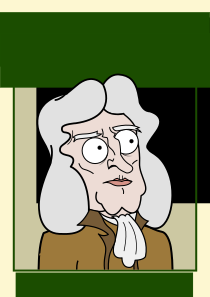
\includepdf{./images/cover/cover-front}

\begin{center}

    \begin{Huge}
    \textbf{Súper libro de Física}
    \end{Huge}

    \vspace{1cm}
    \textbf{Primera edición v0.1}
    \vspace{2cm}

    \begin{Large}
        Malvicino, Maximiliano R. \\
        Bosio, Federico A.
    \end{Large}

\end{center}

\clearpage
\noindent
\textbf{Prefacio}

La versión digital más reciente de este texto es gratis y puede ser descargada de
\begin{center}
    \small
    \url{https://github.com/mrmalvicino/super-libro-de-fisica}
\end{center}

\renewcommand{\spanishappendixname}{Anexo}
\tableofcontents

\mainmatter
\pagenumbering{arabic}


\chapter{Cinemática}

\emph{La cinemática es el estudio del movimiento.}
El movimiento suele describirse mediante tres magnitudes: posición, velocidad y aceleración.
A grandes rasgos, estas magnitudes se comprenden como sigue.
\begin{itemize}
    \item La posición indica dónde está lo que se mueve.
    \item La velocidad indica qué tan rápido se mueve.
    \item La aceleración indica con qué fuerza se mueve.
\end{itemize}

\begin{mdframed}[style=MyFrame2]
    \begin{example}
        \label{eg:mag}
    \end{example}
    \cusTi{Magnitudes cinemáticas}

    Para un auto en el kilómetro 10 de la Ruta Provincial 4, cuyo velocímetro marca \SI{60}{\kilo\meter/\hour}, y cuyo conductor pisa bruscamente el freno:
    \begin{itemize}
        \item La posición del auto se indica en el ``mojón kilométrico'' que, en este caso, está a \SI{10}{km} del lugar en el que nace la ruta.
        \item La velocidad está en los controles indicadores del auto, es decir, el velocímetro, que marca \SI{60}{\kilo\meter/\hour}.
        \item La aceleración está relacionada con la fuerza que sienten los pasajeros del auto cuando el conductor pisa el freno.
        La aceleración de frenado de un automóvil común ronda los \SI{5}{\meter/\second\squared}.
    \end{itemize}

    \begin{center}
        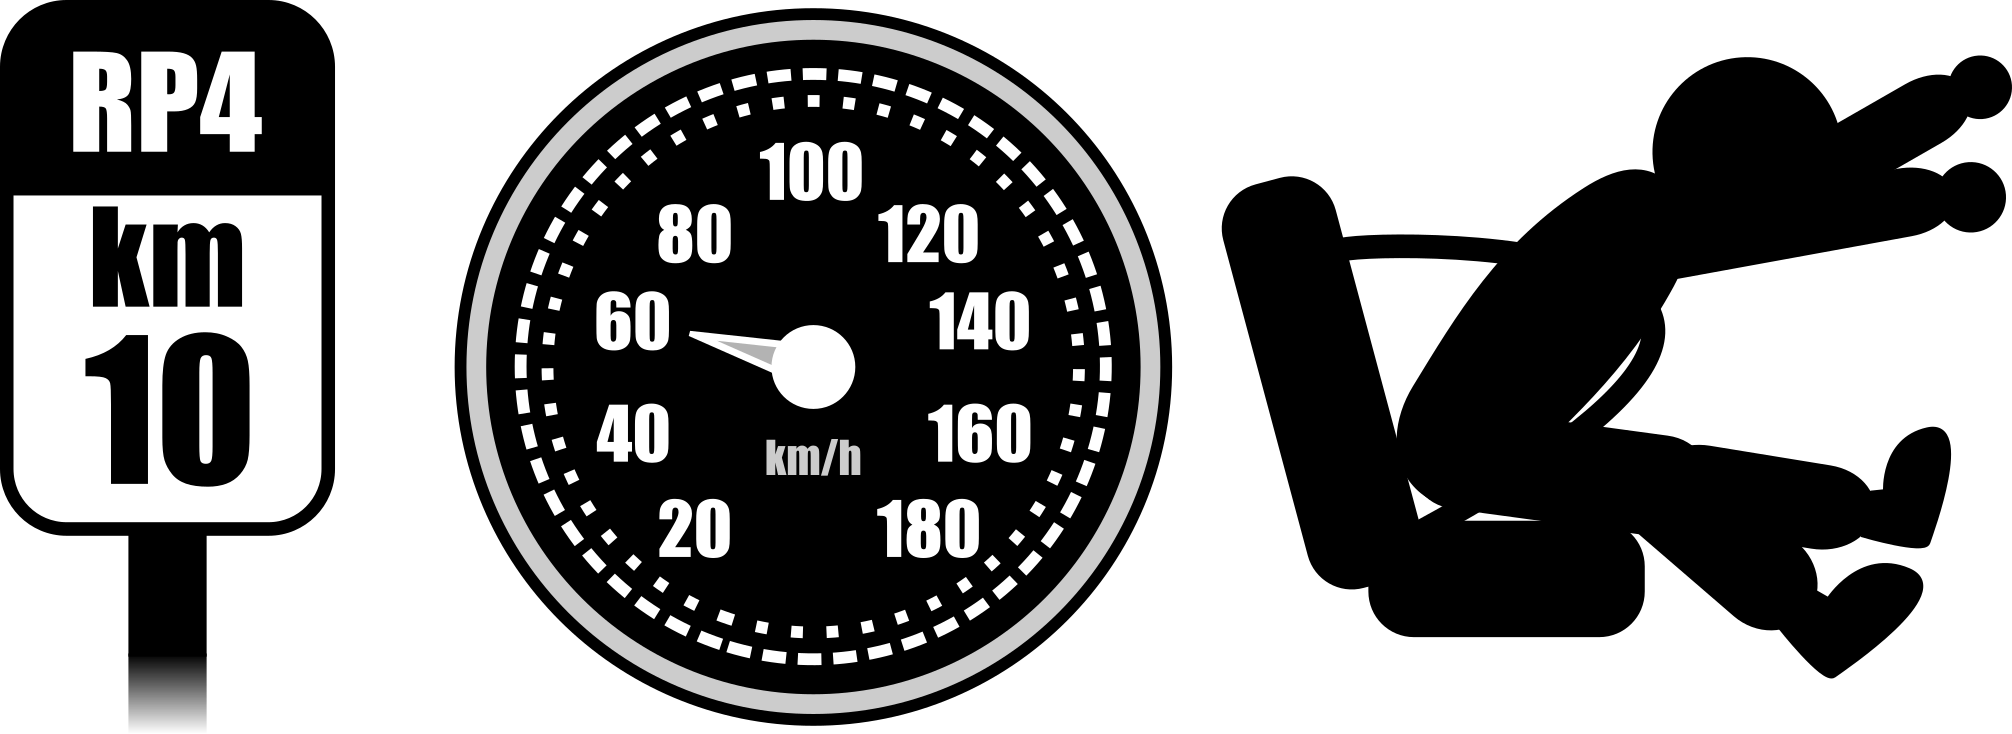
\includegraphics[width=\linewidth]{cinematica-mojon.png}
    \end{center}
\end{mdframed}

En este capítulo, van a estudiarse distintos movimientos que involucran las tres magnitudes.
Cabe destacar que sólo se estudian los movimientos en sí, y no sus causas, que se verán en capítulos posteriores.

\section{Posición, trayectoria y desplazamiento}

La posición se modela matemáticamente como un vector en el espacio, cuyas coordenadas se expresan en un sistema de referencia determinado. En su forma más general, el vector posición se define como sigue.

\begin{mdframed}[style=MyFrame1]
    \begin{defn}
        \label{defn:position}
    \end{defn}
    \cusTi{Función de posición}
    \begin{equation*}
        \xyz(t) = \begin{bmatrix} x(t) & y(t) & z(t) \end{bmatrix}
    \end{equation*}
\end{mdframed}

Todas las coordenadas son funciones del tiempo, lo cual se pone de manifiesto en las $t$ entre paréntesis que aparecen en la notación.
Las relaciones que las componentes del vector posición tienen con la variable $t$ se llaman \emph{ecuaciones horarias}, \emph{ecuaciones de movimiento}, o \emph{ecuaciones paramétricas}.

A veces es necesario usar un vector pero basta con que tenga dos de las tres dimensiones espaciales. La posición de movimientos en dos dimensiones suele denotarse entonces como $\xyz(t)=\sqb{x(t)&y(t)}$ o lo que es lo mismo $\xyz(t)=x(t)\,\iVer + y(t)\,\jVer$ siendo $\iVer$ y $\jVer$ los versores canónicos.

En muchos casos (como en el ejemplo \ref{eg:mag} del auto en la ruta), interesa solamente la distancia a una referencia (el número escrito en el cartel) y en ves de usar un vector $\xyz(t)$ se trabaja con un escalar, generalmente denotado $x(t)$.

Podemos referirnos a una única posición de un cuerpo en un instante de tiempo en particular. Esto es, evaluar dicho instante $t_\ith$ en $\xyz(t)$ para obtener un vector que tiene valores numéricos fijos en sus componentes.

O bien podemos referirnos a todo el recorrido, dado por la imagen de $\xyz(t)$ que traza las sucesivas posiciones por las que pasa el cuerpo conforme transcurre el tiempo. A este recorrido se lo llama \emph{trayectoria}. La trayectoria es el espacio geométrico que ocupan todas las posiciones de un cuerpo en movimiento, dadas por $\xyz(t)$.

En el siguiente gráfico se observa que una \emph{trayectoria} es el conjunto de posiciones sucesivas por las que pasa un cuerpo, mientras que $P_{t_\ith}=\sqb{x(t_\ith)&y(t_\ith)}$ es una de las posiciones que toma el cuerpo a lo largo de su trayectoria.

\begin{center}
    \vspace{-6cm}
    \def\svgwidth{\linewidth}
    \input{./images/cinematica-trayect-1.pdf_tex}
    \vspace{-6cm}
\end{center}  

Para toda trayectoria o fragmento de trayectoria se puede definir el desplazamiento, que es el vector que une el punto inicial con el final. Esto es, la resta entre ambos vectores:

\begin{mdframed}[style=MyFrame1]
    \begin{defn}
        \label{defn:desplazamiento}
    \end{defn}
    \cusTi{Desplazamiento}
    \begin{equation*}
        \Delta \xyz = \xyz(t_F) - \xyz(t_0)
    \end{equation*}
\end{mdframed}

El desplazamiento no debe confundirse con el largo del trayecto recorrido. A continuación se muestran, sobre el gráfico anterior, el vector desplazamiento y el segmento de trayecto considerado en negro oscuro. El segmento estudiado está dado arbitrariamente según se definan los puntos inicial y final.

\begin{center}
    \vspace{-6cm}
    \def\svgwidth{\linewidth}
    \input{./images/cinematica-trayect-2.pdf_tex}
    \vspace{-6cm}
\end{center}

Hay movimientos en dos dimensiones como el tiro oblicuo~(Sec. \ref{subsec:parabolicMotion}) y el movimiento circular~(Sec. \ref{sec:circularMotion}). Estas trayectorias tienen una forma particular y serán estudiadas con más detalle posteriormente. Pero también pueden darse otras menos comunes.

A continuación se muestra un ejemplo de una trayectoria curva que representa el recorrido de un bote en una laguna, visto desde el cielo.

\begin{mdframed}[style=MyFrame2]
    \begin{example}
        \label{eg:boatPosition}
    \end{example}
    \cusTi{Bote en una laguna: Posición}
    \begin{formatI}
        A partir de la siguiente función de posición, describir cualitativamente el movimieto.
    \end{formatI}
    \begin{equation*}
        \xyz:D \subseteq \setR \longrightarrow \setR^2 \tq \xyz(t) = \sqb{t^3\,\si{\metre\per\second^3}, t^2\,\si{\metre\per\second^2}}
    \end{equation*}

    \begin{center}
        \vspace{-5cm}
        \def\svgwidth{\linewidth}
        \input{./images/cinematica-boat-1.pdf_tex}
        \vspace{-6cm}
    \end{center}

Observar que:
    \begin{enumerate}
        \item El vector posición tiene en cada coordenada una función escalar de $t$.
        En este caso, las ecuaciones horarias son $x(t) = t^3\,\si{\metre\per\second^3}$ e $y(t) = t^2\,\si{\metre\per\second^2}$.
        \item La trayectoria curva se da en horizontal sobre la superficie de la tierra, pero una trayectoria en 2~dimensiones puede darse verticalmente, como por ejemplo una hormiga caminando en una pared o una pelota lanzada en diagonal hacia arriba.
        \item Se puede comprobar que, dependiendo de qué valor de tiempo asignemos a la función, obtendremos las coordenadas del bote.
        Las coordenadas indican la posición del bote en la laguna en diferentes instantes de tiempo.
    \end{enumerate}

    Supongamos que el tiempo negativo es el pasado y el tiempo positivo, el futuro, y que el muelle $A$ se encuentra en la coordenada $[x,y] = [-8,4]\,\si{\metre}$ y el muelle $C$ en la coordenada $[x,y] = [8,4]\,\si{\metre}$.
    Entonces deducimos que el bote partió del muelle $A$, se encuentra en el muelle $B$ y se dirige hacia el muelle $C$.
    El muelle $B$ se encuentra en el origen de coordenadas porque, si allí está el bote en el presente, entonces $t = \SI{0}{\minute}$ y, cuando el tiempo toma este valor, se tiene que $\xyz(\SI{0}{\minute}) = [0,0]\,\si{\metre}$.
    Además, concluimos que el bote tardará 4~minutos en hacer todo el recorrido, porque hace 2~minutos estaba en el muelle $A$, pues $\xyz(\SI{-2}{\minute}) = [-8,4]\,\si{\metre}$, y dentro de 2 minutos estará en el muelle $C$, pues $\xyz(\SI{2}{\minute}) = [8,4]\,\si{\metre}$.
\end{mdframed}

Cabe mencionar que la función vectorial ($\xyz$) del ejemplo anterior es inyectiva, ya que cada coordenada $[x,y]$ se obtiene a partir de un único valor del dominio $(t)$.
Una función vectorial no inyectiva pasa dos veces por el mismo lugar, es decir, en dos instantes distintos de tiempo se obtiene el mismo vector de posición.
Si estás pensando en que hay dos valores de $x$ que tienen una misma coordenada $y$ entonces no te estás dando cuenta que tanto $x$ como $y$ son valores de la imagen de la función.


\section{Velocidad y aceleración}

El cambio en la posición va a ir forjando el ``recorrido'' que haga el cuerpo.

Intuitivamente, podemos entender a la velocidad como qué tan rápido cambia la posición de un cuerpo y, análogamente, la aceleración como qué tan rápido cambia su velocidad.

La velocidad media es la razón de cambio promedio de la posición con respecto del tiempo transcurrido.

\begin{mdframed}[style=MyFrame1]
    \begin{defn}
    \end{defn}
    \cusTi{Velocidad media}
    \begin{equation*}
        \media{\Vec{v}}{\left[ t_0 ; t_1 \right]}
      = \dfrac{\Delta \xyz(t)}{\Delta t}
      = \dfrac{\xyz(t_1)-\xyz(t_0)}{t_1-t_0}
    \end{equation*}
\end{mdframed}

Y la aceleración media es la razón de cambio promedio de la velocidad con respecto del tiempo.

\begin{mdframed}[style=MyFrame1]
    \begin{defn}
    \end{defn}
    \cusTi{Aceleración media}
    \begin{equation*}
        \media{\Vec{a}}{\left[ t_0 ; t_1 \right]}
      = \dfrac{\Delta \Vec{v}(t)}{\Delta t}
      = \dfrac{\Vec{v}(t_1)-\Vec{v}(t_0)}{t_1-t_0}
    \end{equation*}
\end{mdframed}

La velocidad y aceleración \emph{media} se diferencian de la velocidad y aceleración \emph{instantánea}, respectivamente, en la forma que lo hacemos a continuación.

Hacer un análisis \emph{instante a instante} significa \emph{estudiar intervalos de tiempo infinitamente cortos}.
Es decir, ya que consideramos el tiempo continuo, entre dos instantes de tiempo determinados hay infinitos instantes que los separan. La aplicación matemática que nos permite hacer este análisis es el límite. Aplicando límite en las definiciones anteriores podemos observar que quedan definidas las derivadas. Coloquialmente, decimos que los $\Delta$ pasan a ser $\dif$.

En Cinemática, la ventaja de trabajar con funciones vectoriales es que derivarlas es muy fácil, ya que se derivan componente a componente:
\[
  \xyz (t) = \begin{bmatrix} x(t) & y(t) \end{bmatrix} \implies
  \dfrac{\dif}{\dif t} \xyz (t) =
  \begin{bmatrix} \dfrac{\dif}{\dif t} x(t) & \dfrac{\dif}{\dif t} y(t) \end{bmatrix}
\]

Por lo tanto, la velocidad está definida como la primera derivada de la posición.
\begin{equation*}
    \Vec{v}\left(t_0\right) = \lim_{t \to t_0} \dfrac{\xyz(t)-\xyz(t_0)}{t-t_0}
\end{equation*}

\begin{mdframed}[style=MyFrame1]
    \begin{defn}
    \end{defn}
    \cusTi{Velocidad (instantánea)}
    \begin{equation*}
        \Vec{v}(t) = \dfrac{\dif}{\dif t} \xyz (t) = \sqb{\dfrac{\dif}{\dif t} x(t) & \dfrac{\dif}{\dif t} y(t)}
    \end{equation*}
\end{mdframed}

Y la aceleración está dada por la primera derivada de la velocidad, o lo que es lo mismo, por la segunda derivada de la posición.
\begin{gather*}
    \Vec{a}\left(t_0\right) = \lim_{t \to t_0} \dfrac{\Vec{v}(t)-\Vec{v}(t_0)}{t-t_0}
    \\
    \Vec{a}(t) =
    \dfrac{\dif}{\dif t} \Vec{v} (t) =
    \dfrac{\dif}{\dif t} \underbrace{\dfrac{\dif}{\dif t} \xyz (t)}_{\Vec{v}(t)}
\end{gather*}

\begin{mdframed}[style=MyFrame1]
    \begin{defn}
    \end{defn}
    \cusTi{Aceleración (instantánea)}
    \begin{equation*}
        \Vec{a}(t) =
        \dfrac{\dif^2}{\dif t^2} \xyz (t) =
        \begin{bmatrix}
            \dfrac{\dif^2}{\dif t^2} x(t) & \dfrac{\dif^2}{\dif t^2} y(t)
        \end{bmatrix}
    \end{equation*}
\end{mdframed}

Para referirse a la velocidad instante a instante, o a la aceleración instante a instante, la palabra ``instantánea'' suele darse por sobreentendida.

\begin{mdframed}[style=MyFrame2]
    \begin{example}
    \end{example}
    \cusTi{Bote en una laguna: Velocidad y aceleración.}
    \begin{formatI}
        Calcular la velocidad y la aceleración a partir de la trayectoria propuesta en el ejemplo \ref{eg:boatPosition}.
    \end{formatI}
    La posición está dada por:
    \begin{equation*}
        \xyz(t) = \sqb{t^3\,\si{\metre\per\second^3}, t^2\,\si{\metre\per\second^2}}
    \end{equation*}

    Haciendo la primera derivada de la trayectoria obtenemos la velocidad:
    \[ \Vec{v}(t) = \sqb{3\,t^2\,\si{\metre\per\second^3}, 2\,t\,\si{\metre\per\second^2}} \]

    Obsérvese que $\Vec{v}(0\,\si{\second}) = [0, 0]\,\si{\metre\per\second}$. La velocidad en el origen es nula. El bote \emph{frena} para invertir el sentido del movimiento: primero va hacia el sur desde el muelle $A$ hasta el muelle $B$ y luego hacia el norte para llegar al muelle $C$. Esto sólo puede lograrse frenando en medio del movimiento.

    Haciendo la segunda derivada de la posición, que es la derivada de la velocidad, obtenemos la aceleración:
    \[ \Vec{a}(t) = \sqb{6\,t\,\si{\metre\per\second^3}, 2\,\si{\metre\per\second^2}} \]

    El hecho de que la aceleración tenga una componente $y$ constante indica la tendencia del bote a cambiar la dirección de su velocidad para que apunte en la dirección positiva del eje $y$.
    Esto es absolutamente consistente con el comportamiento de la velocidad.
    \begin{align*}
        \Vec{v} \left(-2\,\si{\second}\right)
        &= \sqb{3 \left(-2\,\si{\second}\right)^2\,\si{\metre\per\second^3}, 2\left(-2\,\si{\second}\right)\,\si{\metre\per\second^2}}
        \\
        &= \sqb{12, -4}\,\si{\metre\per\second}
        \\[1ex]
        \Vec{v} \left(2\,\si{\second}\right)
        &= \sqb{3 \left(2\,\si{\second}\right)^2\,\si{\metre\per\second^3}, 2 \left(2\,\si{\second}\right)\,\si{\metre\per\second^2}}
        \\
        &= \sqb{12, 4}\,\si{\metre\per\second}
    \end{align*}

    Los resultados lo muestran claramente: la velocidad del bote en el muelle $A$ apunta en dirección de las $y$ negativas (sur) y, en el muelle $C$, en dirección de las positivas (norte).
    Es precisamente la aceleración positiva en $y$ la que produjo este cambio.
\end{mdframed}


\section{Ecuación de movimiento}

Anteriormente se mencionó que la aceleración es la derivada de la velocidad, que a su vez es la derivada de la posición.
En otras palabras, se puede calcular la aceleración a partir de la posición.
De manera inversa, se puede deducir la posición o ecuación de movimiento a partir de las definiciones de velocidad y aceleración:
\[
  \left\{
   \begin{aligned}
    v &= \dfrac{\dif x}{\dif t}
    \\[1ex]
    a &= \dfrac{\dif^2 x}{\dif t^2} =
    \dfrac{\dif}{\dif t} \dfrac{\dif x}{\dif t} =
    \dfrac{\dif v}{\dif t}
   \end{aligned}
  \right.
\]

Coloquialmente, podemos pensar que los $\dif t$ pasan multiplicando al otro miembro en cada ecuación. Formalmente, estamos calculando el diferencial de distancia $\dif x$ y el diferencial de velocidad $\dif v$, que son aproximaciones lineales de $\Delta x$ y $\Delta v$ respectivamente:
\[
  \left\{
    \begin{aligned}
    v \, \dif t &= \dif x
    \\
    a \, \dif t &= \dif v
    \end{aligned}
  \right.
\]

Ahora, integramos respecto de $t$ entre $t_0$ y $t_1$, tomando a $x$ y $v$ como funciones de $t$.
\[
  \left\{
   \begin{aligned}
     \displaystyle\int_{t_0}^{t_1} v \, \dif t &= \displaystyle\int_{x_0}^{x_1} \dif x =
     \left( x \Big|_{x_0}^{x_1} \right) = x_1 - x_0
     \\[1ex]
     \displaystyle\int_{t_0}^{t_1} a \, \dif t &= \displaystyle\int_{v_0}^{v_1} \dif v =
     \left( v \Big|_{v_0}^{v_1} \right) = v_1 - v_0
   \end{aligned}
  \right.
\]
Observar que $x_0$ es la imagen de $x(t_0)$, $x_1$ es la imagen de $x(t_1)$, $v_0$ es la imagen de $v(t_0)$, $v_1$ es la imagen de $v(t_1)$ y $t_1$ puede ser cualquier valor de $t$ mayor que $t_0$.

Haciendo algunos movimientos algebraicos, se tiene:
\[
  \left\{
    \begin{aligned}
    x_1 &= \displaystyle\int_{t_0}^{t_1} v \, \dif t + x_0
    \\[1ex]
    v_1 &= \displaystyle\int_{t_0}^{t_1} a \, \dif t + v_0
    \end{aligned}
  \right.
\]
Como $t_1$ es arbitrario, puede cambiarse por un $t$ genérico, en cuyo caso $x_1$ y $v_1$ pasan a ser, respectivamente, $x$ y $v$, también genéricos.
A su vez, $v$ puede ser expresado como $v(t)$ y $a$ puede ser expresado como $a(t)$.
Esto requiere, no obstante, cambiar las variables de integración para que no coincidan con el extremo superior de las integrales definidas.
Llamemos $u$, por ejemplo, a las variables de integración.
\[
  \left\{
    \begin{aligned}
    x(t) &= \displaystyle\int_{t_0}^{t} v(u) \, \dif u + x_0
    \\[1ex]
    v(t) &= \displaystyle\int_{t_0}^{t} a(u) \, \dif u + v_0
    \end{aligned}
  \right.
\]
Pero las integrales definidas bien pueden ser expresadas como indefinidas, donde $x_0 = x\left(t_0\right)$ y $v_0 = v\left(t_0\right)$ son las constantes de integración, como se mencionó.
\[
  \left\{
    \begin{aligned}
      x(t) &= \displaystyle\int v(t) \, \dif t + x(t_0)
      \\[1ex]
      v(t) &= \displaystyle\int a(t) \, \dif t + v(t_0)
    \end{aligned}
  \right.
\]

Reemplazando $v(t)$ en $x(t)$, por sustitución se tiene:
\[ x(t) = \int \left( \int a(t) \, \dif t + v(t_0) \right) \dif t + x(t_0) \]

Esta ecuación significa que si se conoce la aceleración, la velocidad inicial, y la posición inicial de una partícula, se pueden predecir sus futuras posiciones y velocidades:
\[ x(t) = \iint a(t) \, \dif t^2 + \int v(t_0) \, \dif t + x(t_0) \]

\begin{mdframed}[style=MyFrame1]
    \begin{defn}
        \label{defn:generalMovementEqn}
    \end{defn}
    \cusTi{Ecuación general de movimiento}
    \begin{equation*}
        x(t) = \displaystyle\iint a(t) \, \dif t^2 + v(t_0) (t-t_0)   + x(t_0)
    \end{equation*}
\end{mdframed}

En Cinemática se suele analizar los movimientos de más de una dimensión componente a componente. Por este motivo, conviene quedarnos solo con el caso particular de 1 dimensión (Def. \ref{defn:generalMovementEqn}).

Pero podemos extrapolar $x(t)$ para $n$ dimensiones, particularmente las 3 dimensiones espaciales. El modelado se haría con la siguiente función vectorial que describe la trayectoria de una partícula en el espacio:
\[
  \xyz(t) :
  \left\{
    \begin{aligned}
      x(t) &= \displaystyle\iint a_x(t) \, \dif t^2 + \displaystyle\int v_x(t_0) \, \dif t + x(t_0)
      \\[1ex]
      y(t) &= \displaystyle\iint a_y(t) \, \dif t^2 + \displaystyle\int v_y(t_0) \, \dif t + y(t_0)
      \\[1ex]
      z(t) &= \displaystyle\iint a_z(t) \, \dif t^2 + \displaystyle\int v_z(t_0) \, \dif t + z(t_0)
    \end{aligned}
  \right.
\]

Donde cada una de las funciones escalares $x(t)$, $y(t)$ y $z(t)$ son las componentes del vector posición (Def. \ref{defn:position}).

Podemos definir dos casos particulares usados frecuentemente.
Por un lado, el caso en que la aceleración de la partícula es constante para todos los valores de tiempo que se estén integrando entre $t_0$ y $t_1$. Y por otro lado, el caso en que la velocidad también lo es y la aceleración, además, es nula. De esta forma, se tienen las siguientes definiciones, respectivamente:

\begin{mdframed}[style=MyFrame1]
    \begin{defn}
        \label{defn:cstAccelMovementEqn}
    \end{defn}
    \cusTi{Ec. de movimiento con aceleración constante no nula}
    \begin{equation*}
        x(t) = \dfrac{a}{2}(t-t_0)^2 + v_0(t-t_0) + x_0
    \end{equation*}
\end{mdframed}

\begin{mdframed}[style=MyFrame1]
    \begin{defn}
        \label{defn:cstVelMovementEqn}
    \end{defn}
    \cusTi{Ec. de movimiento con velocidad constante}
    \begin{equation*}
        x(t) = v_0(t-t_0) + x_0
    \end{equation*}
\end{mdframed}


\section{Movimiento rectilíneo}

Se llama así a todo movimiento unidimensional.
Su ecuación está dada por la definición \ref{defn:generalMovementEqn}, que involucra únicamente una función escalar.

\subsection{MRU}

Un cuerpo en movimiento rectilíneo uniforme (o MRU) es aquel que se mueve en línea recta con aceleración nula, y por lo tanto con velocidad constante.

La ecuación de movimiento con velocidad constante (Def.\ \ref{defn:cstVelMovementEqn}) describe la trayectoria de un MRU.

Por ahora, si el lector quiere verificar que si la aceleración es nula entonces la velocidad será constante, puede hacerlo derivando dos veces la trayectoria del MRU. Más adelante, en el capítulo \ref{cha:dinamics}, se enunciará la primera ley de Newton (Def.\ \ref{defn:NewtonFirstLaw}) que generaliza esta situación.

\begin{mdframed}[style=MyFrame2]
    \begin{example}
    \end{example}
    \cusTi{Auto en la ruta a velocidad constante}
    \begin{formatI}
        Un auto conduce un segmento de \SI{2,2}{\kilo\meter} de la ruta~40 en la provincia de Mendoza, entre las calles Araóz y Boedo, donde la ruta es prácticamente recta. El conductor parte del cruce entre la ruta 40 y Boedo y quiere saber a qué velocidad $(v)$ tiene que configurar el piloto automático para hacer la segunda mitad del trayecto, hasta Araóz, en un minuto.
    \end{formatI}
    
    \begin{center}
        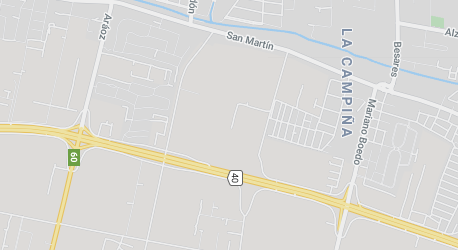
\includegraphics[width=\linewidth]{cinematica-map.png}
    \end{center}
    
    \begin{align*}
        x\left(\SI{60}{\second}\right) &= v \, \SI{60}{\second} + \SI{1100}{\metre} = \SI{2200}{\metre}
        \\[1ex]
        v &= \dfrac{\SI{2200}{\metre}-\SI{1100}{\metre}}{\SI{60}{\second}}
        = \dfrac{\SI{1100}{\metre}}{\SI{60}{\second}}
        = \dfrac{\SI{55}{\metre}}{\SI{3}{\second}}
        \\[1ex]
        &= \dfrac{55 \cdot \frac{1}{1000}\si{\kilo\meter}}{3 \cdot \frac{1}{3600}\si{\hour}}
        = \SI{66}{\kilo\metre/\hour}
    \end{align*}
    
    El sistema de referencia está planteado para que la función de posición tenga origen en el comienzo del segmento de la ruta, es decir, en el cruce de la ruta 40 con Boedo.
    
    \begin{center}
        \vspace{-5cm}
        \def\svgwidth{\linewidth}
        \input{./images/cinematica-map-2.pdf_tex}
        \vspace{-6cm}
    \end{center}
    
    Sería posible resolver el problema, de manera más sencilla (aunque menos general) estableciendo el origen en el medio del segmento de ruta y en este caso la posición inicial sería \SI{0}{\metre} y la posición final $(x_1)$ sería \SI{1100}{\metre}.
    
    El mapa 2 tiene dimensiones, pero como el movimiento se da en línea recta, basta con una coordenada para calcular la trayectoria. Sería innecesario y engorroso (aunque posible) plantear una trayectoria recta de 2 dimensiones para describir el movimiento en el plano $xy$. Cualquier movimiento, en particular uno rectilíneo, puede expresarse con una trayectoria vectorial de 3 dimensiones.
    Pero si se elige correctamente el sistema de referencia, basta con usar 1 dimensión, porque lo que importa es la variación de la distancia.
\end{mdframed}

\begin{mdframed}[style=MyFrame2]
    \begin{example}
    \end{example}
    \cusTi{Dos autos en sentido opuesto}
    \begin{formatI}
        Para este problema de \emph{encuentro}, determinar cuándo y dónde se cruzan los móviles del siguiente esquema.
    \end{formatI}
    
    \begin{center}
        \vspace{-5cm}
        \def\svgwidth{\linewidth}
        \input{./images/cinematica-cars-1.pdf_tex}
        \vspace{-6cm}
    \end{center}
    
    En particular, acá se tienen dos autos en sus respectivos carriles y sentidos opuestos entre sí, separados por una distancia de \SI{300}{\kilo\meter}.
    Uno tiene una velocidad de \SI{50}{\kilo\meter/\hour} y el otro, de \SI{100}{\kilo\meter/\hour}.
    Se busca, como todo problema de encuentro, el instante de tiempo y la posición en que se cruzan.
    
    Tomemos el siguiente sistema de referencia.
    
    \begin{center}
        \vspace{-8cm}
        \def\svgwidth{\linewidth}
        \input{./images/cinematica-cars-2.pdf_tex}
        \vspace{-6cm}
    \end{center}
    
    El origen ($O$) coincide con la posición inicial del auto ubicado en la parte superior del dibujo ($A$).
    De acuerdo al sistema elegido, la posición crece positivamente cuando nos alejamos de $O$ para ir a la posición inicial del auto en el carril inferior ($B$).
    Además, por simplicidad, elegiremos $t_0 = 0$ en el punto $O$, es decir, el inicio del movimiento sucederá cuando el auto A esté ubicado en el punto $O$ del eje $x$.
    
    Con esto ya podemos construir las ecuaciones de movimiento.
    Si adjuntamos a cada $x$ un subíndice correspondiente a cada auto ($A$ o $B$), quedan
    \begin{align*}
        x_A(t) &= 50\,\si{\kilo\metre\per\hour} \, t
        \\
        x_B(t) &= 300\,\si{\kilo\metre} - 100\,\si{\kilo\metre\per\hour} \, t
    \end{align*}
    
    Los signos de las velocidades respetan el sentido de crecimiento del eje $x$: la velocidad de $A$ es positiva porque apunta, en el dibujo, hacia la derecha (como el eje $x$), y la velocidad de B es negativa porque apunta hacia la izquierda (contrario al eje $x$).
    
    Recordemos que, en el instante en que los autos se cruzan, están en la misma posición (en lo que respecta al eje $x$).
    Por eso basta con igualar $x_A$ y $x_B$:
    \[ 50\,\si{\kilo\metre\per\hour} \, t = 300\,\si{\kilo\metre} - 100\,\si{\kilo\metre\per\hour} \, t \]
    
    y ahora sencillamente despejamos $t$
    \[ 150\,\si{\kilo\metre\per\hour} \, t = 300\,\si{\kilo\metre}
    \iff t = \frac{300}{150}\,\si{\hour} = 2\,\si{\hour} \]
    
    Reemplazando en cualquiera de las dos ecuaciones de movimiento, queda
    \[ x_A(2\,\si{\hour}) = 100\,\si{\kilo\metre} = x_B(2\,\si{\hour}) \]
    es decir, los autos se cruzan a las \SI{2}{\hour} de haber iniciado el recorrido, \SI{100}{\kilo\meter} a la derecha del origen.
\end{mdframed}


\subsection{MRUV}

Un cuerpo en movimiento rectilíneo uniformemente variado es aquel que se mueve en línea recta con aceleración constante no nula.

La ecuación de movimiento con aceleración constante (Def. \ref{defn:cstAccelMovementEqn}) describe la trayectoria de los MRUV.

Dependiendo de la naturaleza de la aceleración, podemos distinguir los movimientos dados por la aceleración gravitatoria de los que son acelerados de manera arbitraria por un agente externo.

La diferencia entre los MRUV con aceleración gravitatoria $(g)$ y aquellos con aceleración arbitraria $(a)$ es que $g$ tiene un valor predefinido y conocido mientras que $a$ puede tomar un valor diferente dependiendo de cada situación.

\begin{itemize}
    \item El efecto de la gravedad a escala visible es evidente: si dejo caer un objeto desde cierta altura, su velocidad aumenta cada vez más, lo cual significa que el objeto está acelerado. La aceleración de una partícula debido al campo gravitatorio de la Tierra vale $a = g \approx \SI{9,8}{\metre/\second\squared}$.

    \item El efecto de un agente externo acelerando un cuerpo (como, por ejemplo, un motor acelerando un auto) no es tan trivial. A continuación se dan algunos ejemplos aunque más adelante, para hacer un estudio más exhaustivo, se enunciará la segunda ley de Newton (Def.\ \ref{defn:NewtonSecondLaw}) que permite dar otro enfoque.
\end{itemize}

\begin{mdframed}[style=MyFrame2]
    \begin{example}
    \end{example}
    \cusTi{Auto en la ruta con aceleración constante}
    \begin{formatI}
        Calcular el tiempo que tarda un auto en acelerar de \SI{0}{\kilo\meter\per\hour} a \SI{100}{\kilo\meter\per\hour} si tiene una aceleración $(a)$ de $\num{0,3}\,g$ a lo largo de una ruta recta. Luego, calcular la longitud $(L)$ del segmento de ruta que recorrió en ese tiempo.
    \end{formatI}
    \begin{gather*}
        a = \num{0,3}\,g = \num{0,3} \left( \SI{9,8}{\metre\per\second\squared} \right) = \SI{2,94}{\metre\per\second\squared}
        \\[1ex]
        v(t_1) = \SI{2,94}{\metre\per\second\squared} \, t_1
        \\
        v(t_1) = \SI{100}{\kilo\metre\per\hour}
        = \dfrac{250}{9} \, \si{\metre\per\second}
        \\[1ex]
        t_1 = \dfrac{\frac{250}{9} \, \si{\metre\per\second}}{\SI{2,94}{\metre\per\second\squared}}
        \approx \SI{9,4}{\metre\second\squared\per\metre\per\second}
        = \SI{9,4}{\second}
        \\[1ex]
        x(t_1) =  \frac{a}{2} \, t_1^2 + v_0 \, t_1 + x_0  =  L
        \\
        L =  \dfrac{\SI{2,94}{\metre\per\second\squared}}{2}t_1^2 \approx \SI{130}{\metre}
    \end{gather*}
\end{mdframed}

\begin{mdframed}[style=MyFrame2]
    \begin{example}
    \end{example}
    \cusTi{Nave espacial despegando}
    \begin{formatI}
        Una nave espacial mantiene una aceleración de $\num{1,8}\,g$ desde su despegue hasta que sale de la atmósfera terrestre después de 10 minutos. Verificar que la velocidad que tiene la nave al finalizar ese trayecto, es menor a la velocidad máxima del Falcon 9 Heavy de SpaceX, la cual se estima en~\SI{39600}{\kilo\metre/\hour}.
    \end{formatI}
    \begin{align*}
        a &= \num{1,8}\,g = 17,64 \, \si{\metre\per\second\squared} \implies
        \\
        v \left(\SI{600}{\second}\right) &= \left(\SI{17,64}{\metre\per\second\squared}\right) \SI{600}{\second}
        \\
        &= \SI{10584}{\metre\per\second}
        \\
        &= \SI{38102,4}{\kilo\metre\per\hour} < \SI{39600}{\kilo\metre\per\hour}
    \end{align*}
\end{mdframed}


\subsection{Caída libre}

En esta situación, un cuerpo puntual cae desde cierta altura $(h)$, medida desde el piso, y adquiere una aceleración de magnitud $g$ y sentido hacia abajo. Tanto el movimiento como la aceleración son hacia abajo. Esto no es menor, y se tiene que ver reflejado en la ecuación, de acuerdo al sistema de referencia que se tome.

La caída libre es un tipo de MRUV, por lo que la trayectoria va a ser modelada por la ecuación de movimiento con aceleración constante (Def.\ \ref{defn:cstAccelMovementEqn}) tomando las siguientes consideraciones.

Como el cuerpo parte del reposo, la velocidad inicial es $v_0 = \SI{0}{\metre/\second}$. Si elegimos un sistema orientado positivamente hacia arriba y con el origen en el piso, la posición inicial $\left( x_0 \right)$ va a ser igual a $h$ y la aceleración $(a)$ va a ser negativa:

\begin{mdframed}[style=MyFrame1]
    \begin{defn}
    \end{defn}
    \cusTi{Función de posición de caída libre}
    \begin{equation*}
        y(t) = -\frac{g}{2} \left(t-t_0\right)^2 + h
    \end{equation*}
\end{mdframed}


\subsection{Tiro vertical}

En esta situación un cuerpo puntual cae desde cierta altura $(h)$ y adquiere aceleración gravitatoria $(g)$ con sentido hacia abajo. Pero además, al inicio del movimiento el cuerpo tiene una velocidad inicial $(v_0)$.

Al igual que la caída libre, el tiro vertical se modela con la ecuación de movimiento con aceleración constante (Def.\ \ref{defn:cstAccelMovementEqn}), ya que también es un caso particular de MRUV.

Ahora bien, en este caso se va a mantener el término lineal para incorporar el dato de la velocidad inicial, siendo su signo positivo si, al inicio del movimiento, el cuerpo estaba subiendo, y negativo si estaba bajando.

\begin{mdframed}[style=MyFrame1]
    \begin{defn}
    \end{defn}
    \cusTi{Función de posición del tiro vertical}
    \begin{equation*}
        y(t) = -\frac{g}{2}(t-t_0)^2 \pm v_0(t-t_0) + h
    \end{equation*}
\end{mdframed}


\section{Movimiento curvilíneo}

Hasta ahora se vieron situaciones en las que se daba un movimiento que podía ser acelerado o no, pero siempre era en línea recta. Por este motivo, usábamos la ecuación de movimiento en una dimensión (Def.\ \ref{defn:generalMovementEqn}) y sus casos particulares. Si queremos estudiar una trayectoria curva, necesitamos una parametrización de dos dimensiones. Esto implica que la posición, la velocidad y la aceleración van a considerarse magnitudes vectoriales, y ya no escalares. Para estudiar un movimiento curvilíneo, hay que analizar cómo estas magnitudes son afectadas en cada dimensión, descomponiéndolas.


\section{Tiro oblicuo}
\label{subsec:parabolicMotion}

En esta situación, un cuerpo puntual es arrojado en diagonal con cierto ángulo $(\theta)$ y cierta velocidad inicial $(\Vec{v_0})$ de módulo $\nnorm{\Vec{v_0}} = v_0$. Al descomponer el movimiento para analizar cómo va a variar la cinemática en cada dimensión, podemos observar que:
\begin{itemize}
    \item El eje $z$ no es necesario, ya que si despreciamos cualquier desvío causado por el viento empujando al cuerpo, el movimiento se modela sobre un plano, en dos dimensiones.
    
    \item La trayectoria del cuerpo se va a curvar por la gravedad. Pero esta aceleración solo va a afectar el eje $y$ del movimiento, como si de un tiro vertical se tratase. Por lo tanto, la coordenada vertical de la posición estará dada por la ecuación de movimiento con aceleración constante (Def.\ \ref{defn:cstAccelMovementEqn}).
    
    \item El eje $x$ no se ve afectado por aceleración alguna. Con lo cual, la coordenada horizontal de la posición estará dada por la ecuación de movimiento con velocidad constante (Def.\ \ref{defn:cstVelMovementEqn}). La velocidad en $x$ será contantemente $v_{0x}$, que es aquella impuesta inicialmente por la velocidad inicial.
\end{itemize}

A partir de este análisis, podemos definir la aceleración que rige el movimiento:
\begin{equation*}
    \Vec{a}(t) = \sqb{0 \, , \, -g}
\end{equation*}

Y así también la velocidad, que surge al integrar la aceleración:
\begin{equation*}
    \Vec{v}(t) = \sqb{v_{0x} \, , \, -g \left(t-t_0\right) + v_{0y}}
\end{equation*}

Obteniendo así la posición al integrar nuevamente.

\begin{mdframed}[style=MyFrame1]
    \begin{defn}
    \end{defn}
    \cusTi{Función de posición del tiro oblicuo}
    \begin{equation*}
        \scale{0.92}{
        \xyz(t) = \sqb{v_{0x} \left(t-t_0\right) \, , \, \frac{-g}{2} \left(t-t_0\right)^2 + v_{0y} \left(t-t_0\right) + y_0}
        }
    \end{equation*}
\end{mdframed}

Veamos la fórma que tiene el recorrido de un cuerpo arrojado en tiro oblicuo.

Como estamos estudiando un único cuerpo podemos establecer $t_0=\SI{0}{\second}$ ya que para estudiar una única trayectoria no es necesario considerar un retraso temporal. Las coordenadas $x(t)$ e $y(t)$ del vector $\xyz(t) = \sqb{x(t),y(t)}$ quedan entonces dadas por:
\begin{equation*}
    \left\{
    \begin{aligned}
        x(t) &= v_{0x} \, t
        \\
        y(t) &= -\frac{g}{2} \, t^2 + v_{0y} \, t + y_0
    \end{aligned}
    \right.
\end{equation*}

Despejando el parámetro $t$ de la primer ecuación y reemplazándolo en la segunda, se tiene:
\begin{align}
    y &= -\frac{g}{2} \, \left(\frac{x}{v_{0x}}\right)^2 + v_{0y} \left(\frac{x}{v_{0x}}\right) + y_0
    \notag
    \\
    y(x) &= -\frac{g}{2 \, v_{0x}^2} \, x^2 + \frac{v_{0y}}{v_{0x}} \, x + y_0
    \label{eqn:oblicuoCurva}
\end{align}

Luego, es esperable que la trayectoria de la partícula sea una parábola invertida.

A continuación, se muestra un gráfico con las implicaciones geométricas en la trayectoria del movimiento.
Notar que se está graficando, en un mismo gráfico, la trayectoria y la velocidad de la partícula en ciertos puntos de la misma.
El largo de las flechas, indica la magnitud del vector.

\begin{center}
    \vspace{-5cm}
    \def\svgwidth{\linewidth}
    \input{./images/cinematica-tiro-oblicuo-1.pdf_tex}
    \vspace{-6cm}
\end{center}

Donde:
\begin{align*}
    v_{0x} &= v_0 \cos(\theta)
    \\
    v_{0y} &= v_0 \sin(\theta)
\end{align*}

Concluyendo que:

\begin{itemize}
    \item La componente vertical de la velocidad $(v_y)$ va disminuyendo hasta que se hace nula en el punto $\sqb{x_h, y_h}$, donde la altura es máxima y el módulo de la velocidad es mínimo (pero no nulo).
    
    \item El módulo de la velocidad es máximo en el punto donde la altura es mínima $(y=\SI{0}{\metre})$. Esto sucede al final del recorrido, justo antes de que el cuerpo choque contra el piso.
    
    \item Para todos los pares de puntos donde la altura es la misma, la velocidad tiene el mismo módulo y el vector velocidad forma el mismo ángulo con el eje $x$ pero hacia abajo.
    
    \item La componente horizontal de la velocidad $(v_x)$ es constante para todos los puntos de la trayectoria.
\end{itemize}

Cuando se estudian las posibles trayectorias de un tiro oblicuo, suele ser de interés calcular el \emph{alcance} que va a tener el cuerpo. Esta distancia $x_d$ para la cual el cuerpo impacta en el piso está dada para el punto cuya coordenada vertical es nula.

Así, al igualar a cero la ecuación \ref{eqn:oblicuoCurva} se tiene, completando cuadrados:
\begin{align*}
    0 &= -\frac{g}{2 \, v_{0x}^2} \, x^2 + \frac{v_{0y}}{v_{0x}} \, x + y_0
    \\[1ex]
    &= x^2 - \frac{2 \, v_{0x}^2}{g} \frac{v_{0y}}{v_{0x}} \, x - \frac{2 \, v_{0x}^2}{g} \, y_0
    \\[1ex]
    &= x^2 - 2 \, \frac{v_{0x} \, v_{0y}}{g} \, x - \frac{2 \, v_{0x}^2}{g} \, y_0
    \\[1ex]
    &= \left(x - \frac{v_{0x} \, v_{0y}}{g}\right)^2 - \left(\frac{v_{0x} \, v_{0y}}{g}\right)^2 - \frac{2 \, v_{0x}^2}{g} \, y_0
\end{align*}

Entonces, si consideramos $y_0=\SI{0}{\metre}$ como un caso particular, el alcance es:
\begin{align*}
    \left(x - \frac{v_{0x} \, v_{0y}}{g}\right)^2 &= \left(\frac{v_{0x} \, v_{0y}}{g}\right)^2
    \\[1ex]
    x &= \frac{2 \, v_{0x} \, v_{0y}}{g}
    \\[1ex]
    &= \frac{2 \cos(\theta) \sin(\theta) \, v_0^2}{g}
\end{align*}

Y, finalmente, usando la propiedad trigonométrica del seno de ángulo doble que implica $2 \cos(\theta) \sin(\theta)=\sin(2\theta)$ se obtiene

\begin{mdframed}[style=MyFrame1]
    \begin{prop}
        \label{prop:oblicuoAlcance}
    \end{prop}
    \cusTi{Alcance de tiro oblicuo}
    \begin{equation*}
        y_0 = \SI{0}{\metre} \implies x_d = \frac{\sin(2\theta) \, v_0^2}{g}
    \end{equation*}
\end{mdframed}

Aunque podríamos usar las parametrizaciones $x(t)$ e $y(t)$ para dar con una fórmula para el alcance que admita $y_0 \neq \SI{0}{\metre}$. Primero se calcula el tiempo $t=t_d$ tal que $y(t)=\SI{0}{\metre}$ siendo este lo que tarda el cuerpo en tener altura nula. Completando cuadrados esto es:
\begin{align*}
    0 &= -\frac{g}{2} \, t^2 + v_{0y} \, t + y_0
    \\[1ex]
    &= t^2 - 2 \, \frac{v_{0y}}{g} \, t - \frac{2\,y_0}{g}
    \\[1ex]
    &= \left( t - \frac{v_{0y}}{g} \right)^2 - \left(\frac{v_{0y}}{g}\right)^2 - \frac{2\,y_0}{g}
    \\[1ex]
    \left( t - \frac{v_{0y}}{g} \right)^2 &= \left(\frac{v_{0y}}{g}\right)^2 + \frac{2\,y_0}{g}
    \\[1ex]
    t>\frac{v_{0y}}{g} \implies t_d &= \sqrt{\left(\frac{v_{0y}}{g}\right)^2 + \frac{2\,y_0}{g}} + \frac{v_{0y}}{g}
\end{align*}

Y luego se evalúa $x(t_d)$ para obtener el alcance:
\begin{align*}
    x_d &= v_{0x} \, t_d
    \\[1ex]
    &= \sqrt{v_{0x}^2} \sqrt{\left(\frac{v_{0y}}{g}\right)^2 + \frac{2\,y_0}{g}} + \frac{v_{0x}\,v_{0y}}{g}
    \\[1ex]
    &= \sqrt{\left(\frac{v_{0x}\,v_{0y}}{g}\right)^2 + \frac{2 \, y_0 \, v_{0x}^2}{g}} + \frac{v_{0x}\,v_{0y}}{g}
\end{align*}

O bien, usando trigonometría podemos expresar el resultado en función de la norma de la velocidad inicial ($v_0$) y el ángulo ($\theta$) que forma con la horizontal.
\begin{multline*}
    x_d = \sqrt{\left(\frac{v_0^2 \cos(\theta) \sin(\theta)}{g}\right)^2 + \frac{2 \, y_0 \, v_0^2 \cos^2(\theta)}{g}} +
    \\ + \frac{v_0^2 \cos(\theta) \sin(\theta)}{g}
\end{multline*}

Y, finalmente, usando la propiedad trigonométrica del seno de ángulo doble se obtiene

\begin{mdframed}[style=MyFrame1]
    \begin{prop}
    \end{prop}
    \cusTi{Alcance de tiro oblicuo}
    \begin{equation*}
        \scale{0.94}{
        x_d = \sqrt{\left(\frac{\sin(2\theta) \, v_0^2}{2g}\right)^2 + \frac{2 \, y_0 \, v_0^2 \cos^2(\theta)}{g}} + \frac{\sin(2\theta) \, v_0^2}{2g}
        }
    \end{equation*}
\end{mdframed}

A partir de cualquiera de ambas propiedades podemos estudiar el alcance en función del ángulo de tiro tomando un valor fijo para $v_0$.

Para el caso en que $y_0 = \SI{0}{\metre}$ se puede usar la propiedad \ref{prop:oblicuoAlcance} para estudiar $x_d$ en función de $\theta$ como sigue.
\begin{equation*}
    x_d = \frac{\sin(2\theta) \, v_0^2}{g}
\end{equation*}

El gráfico de la función $\sin(2\theta)$ está acotado tal que
\begin{equation*}
    0 \leq \theta \leq \ang{90} \Rightarrow 0 \leq x_d \leq \frac{v_0^2}{g}
\end{equation*}

Y presenta un máximo en $\theta=\pi/4$. Lo cual significa que el alcance $x_d$ va a tomar un valor de $v_0^2/g$ como máximo cuando el ángulo de tiro sea $\ang{45}$. Además, dado que las funciones senoidales son simétricas con respecto a un máximo, vemos que el alcance va a ser el mismo para ángulos simétricos con respecto de $\ang{45}$. Esto se traduce en la siguiente propiedad.

\begin{mdframed}[style=MyFrame1]
    \begin{prop}
    \end{prop}
    Sea $\alpha>0$ el módulo de la diferencia entre $\ang{45}$ y el ángulo de tiro ($\theta$). Para el caso $y_0 = \SI{0}{\metre}$ de tiro oblicuo se tiene que
    \begin{equation*}
        x_d(\theta_1) = x_d(\theta_2) \iff \theta_{1,2} = \ang{45} \pm \alpha
    \end{equation*}
\end{mdframed}

A continuación podemos ver un gráfico que ilustra estas conclusiones. En él se muestran algunas de las posibles trayectorias de un tiro oblicuo en función de una velocidad inicial con ángulo variable pero de norma constante.

\begin{center}
    \vspace{-5cm}
    \def\svgwidth{\linewidth}
    \input{./images/cinematica-tiro-oblicuo-2.pdf_tex}
    \vspace{-6cm}
\end{center}


\section{Movimiento circular}
\label{sec:circularMotion}

El movimiento circular es otro caso particular de movimiento curvilíneo. En un movimiento curvilíneo cualquiera, un cuerpo puede tener una trayectoria errática. En cambio, la trayectoria de un cuerpo en movimiento circular está delimitada por un círculo.

El inconveniente a la hora de deducir ecuaciones horarias para describir la posición de la partícula es que no es posible identificar un valor de aceleración constante en ninguno de los ejes cartesianos, tal como se hacía por ejemplo para un tiro verical donde se podía afirmar que $a_x=\SI{0}{\metre\per\second^2}$ y $a_y=-g\,\si{\metre\per\second^2}$. Es por esto que es necesario usar {coordenadas polares} para referir las magnitudes a estudiar. Ver sección \ref{A:polarCoordinates} del anexo.

A continuación, se muestra el gráfico de una trayectoria circular para una partícula, representada por un punto negro, junto con la posición y sus componentes cartesianas, la velocidad que tiene en ese punto, y las aceleraciones que pueden estar afectando el movimiento.

\begin{center}
    \vspace{-5cm}
    \def\svgwidth{\linewidth}
    \input{./images/cinematica-circular-1.pdf_tex}
    \vspace{-6cm}
\end{center}

La posición $(\xyz)$ se puede expresar como un vector que rota con un extremo fijo en el centro del círculo, como la aguja de un reloj. Las componentes del vector cambian conforme pasa el tiempo. Pero el largo del vector posición es siempre el mismo, y es equivalente al radio $(r)$ del círculo.

\begin{mdframed}[style=MyFrame1]
    \begin{prop}
        \label{prop:circularMovRadius}
    \end{prop}
    \cusTi{Radio del movimiento circular}
    \begin{equation*}
        r = \nnorm{\xyz(t)}
    \end{equation*}
\end{mdframed}

En un movimiento curvilíneo cualquiera, la velocidad ``neta'' puede definirse a partir de la suma entre las velocidades tangencial y radial.

\begin{mdframed}[style=MyFrame1]
    \begin{defn}
    \end{defn}
    \cusTi{Velocidad en polares}
    \begin{equation*}
        \Vec{v} = \Vec{v}_t + \Vec{v}_r
    \end{equation*}
\end{mdframed}

Además, la velocidad de un cuerpo tiene que ser tangente a su trayectoria en todo momento. Pero no hay que confundir la naturaleza tangencial de la velocidad con respecto a la trayectoria con la componente tangencial de la velocidad, que hace referencia a la ortogonalidad entre el vector velocidad y el radio de la circunferencia que pasa por un punto de la trayectoria. En la siguiente imagen vemos una trayectoria curvilínea cualquiera (en línea punteada) sobre la que se grafican los vectores velocidad para dos posiciones distintas.

\begin{center}
    \vspace{-5cm}
    \def\svgwidth{\linewidth}
    \input{./images/cinematica-circular-2.pdf_tex}
    \vspace{-6cm}
\end{center}

En ambos puntos la velocidad es tangencial a la trayectoria, pero solo $\vec{v}_1$ es ortogonal a la dirección radial del círculo de referencia.

La componente radial de la velocidad impone cómo tiende a darse la trayectoria hacia adentro o hacia afuera del círculo de referencia. Si existiese una componente radial de velocidad se podría formar una trayectoria espiral, por ejemplo.

Pero $\nnorm{\Vec{v}_r} = \SI{0}{\metre\per\second}$ ya que para que la trayectoria sea circular se tiene que cumplir la siguiente propiedad.

\begin{mdframed}[style=MyFrame1]
    \begin{prop}
        \label{prop:circularMovVel}
    \end{prop}
    \cusTi{Velocidad del movimiento circular}
    \begin{equation*}
        \Vec{v} = \Vec{v}_t
    \end{equation*}
\end{mdframed}

Un cuerpo en movimiento circular está sometido a una aceleración radial $(\vec{a}_r)$ o centrípeta $(\Vec{a}_c)$ en todo momento. Esta apunta hacia el centro y su magnitud es tal que contrarresta la tendencia ``natural'' del cuerpo a tener una trayectoria recta. Cabe aclarar que la aceleración radial es la misma que la centrípeta: solo se diferencian por ser opuestas en su notación.

El movimiento circular puede o no tener aceleración tangencial $(\Vec{a}_ t)$. La aceleración tangencial puede ser positiva o negativa, dependiendo de la situación. De existir, esta hace que el cuerpo se mueva cada vez más (o menos) rápido sobre el círculo.

\begin{mdframed}[style=MyFrame1]
    \begin{defn}
    \end{defn}
    \cusTi{Aceleración en polares}
    \begin{equation*}
        \Vec{a} = \Vec{a}_t + \Vec{a}_r = \Vec{a}_t - \Vec{a}_c
    \end{equation*}
\end{mdframed}

A medida que el ángulo $(\theta)$ aumenta o disminuye en sentido horario o antihorario, la partícula se mueve por la circunferencia trazando un arco de círculo de cierto largo $(s)$. Es evidente que para que la partícula se mueva, el ángulo va a cambiar conforme pase el tiempo. Ergo, el ángulo es una función escalar del tiempo.

Es determinante qué tan rápido aumenta o disminuye el ángulo. La tasa de cambio del ángulo con respecto del tiempo se conoce como velocidad angular $(\omega)$.

\begin{mdframed}[style=MyFrame1]
    \begin{defn}
        \label{defn:angularVel}
    \end{defn}
    \cusTi{Velocidad angular}
    \begin{equation*}
        \omega (t) = \dfrac{\dif}{\dif t} \theta (t)
    \end{equation*}
\end{mdframed}

Con el mismo criterio, se define la aceleración angular $(\alpha)$ como la derivada de la velocidad angular con respecto del tiempo.

\begin{mdframed}[style=MyFrame1]
    \begin{defn}
        \label{defn:angularAccel}
    \end{defn}
    \cusTi{Aceleración angular}
    \begin{equation*}
        \alpha (t) = \dfrac{\dif}{\dif t} \omega (t) = \dfrac{\dif^2}{\dif t^2} \theta (t)
    \end{equation*}
\end{mdframed}

La velocidad angular está relacionada con la velocidad tangencial, y de igual manera la aceleración angular lo está con la aceleración tangencial. Pero no son lo mismo. Veamos cómo se relacionan.

Dividiendo por el incremento $\Delta t$ y luego tomando el límite cuando $\Delta t \to 0$ en la definición de longitud de arco (Sec. \ref{A:arcLength}) se tiene:
\begin{align*}
    \Delta s &= \Delta \theta \, r
    \\[1ex]
    \frac{\Delta s}{\Delta t} &= \frac{\Delta \theta}{\Delta t} \, r
    \\[1ex]
    \frac{\dif s}{\dif t} &= \frac{\dif \theta}{\dif t} \, r
\end{align*}

La derivada de la izquierda es la velocidad tangencial. Indica qué tan rápido crece el largo de arco de la circunferencia. La derivada de la derecha es la velocidad angular. Indica qué tan rápido aumenta el ángulo. Se obtiene así una relación entre la velocidad angular (Def.\ \ref{defn:angularVel}) y la velocidad tangencial ($v_t$).

\begin{mdframed}[style=MyFrame1]
    \begin{prop}
        \label{prop:circularVel}
    \end{prop}
    \begin{equation*}
        v_t(t) = \omega(t) \, r
    \end{equation*}
\end{mdframed}

Derivando nuevamente, de manera similar se relaciona la aceleración angular (Def.\ \ref{defn:angularAccel}) con la tangencial ($a_t$).

\begin{mdframed}[style=MyFrame1]
    \begin{prop}
        \label{prop:circularAccel}
    \end{prop}
    \begin{equation*}
        a_t(t) = \alpha(t) \, r
    \end{equation*}
\end{mdframed}

A partir de las conclusiones anteriores, siguiendo el mismo razonamiento que se usó para definir la ecuación de movimiento (Def. \ref{defn:generalMovementEqn}), se define la variación del ángulo en función del tiempo o \emph{posición angular}.

\begin{mdframed}[style=MyFrame1]
    \begin{defn}
        \label{defn:anglePosition}
    \end{defn}
    \cusTi{Posición angular}
    \begin{equation*}
        \theta(t) = \iint \alpha(t) \, \dif t^2 + \omega (t_0) \left(t-t_0\right) + \theta(t_0)
    \end{equation*}
\end{mdframed}


\subsection{MCU}
El movimiento circular es \emph{uniforme} cuando el cuerpo gira en torno a la circunferencia con \emph{velocidad angular constante}.

El MCU hereda las propiedades \ref{prop:circularMovRadius} y \ref{prop:circularMovVel} generales para movimientos circulares. A saber:
\begin{itemize}
    \item Al ser un movimiento circular, el radio permanece constante.
    
    \item La velocidad radial es nula y, en consecuencia, el vector velocidad sólo tiene la componente tangencial.
\end{itemize}

Además, se incorporan las siguientes propiedades particulares del MCU.

Como la velocidad angular y el radio son constantes, el módulo de la velocidad también lo es, de acuerdo a la propiedad \ref{prop:circularVel}.

\begin{mdframed}[style=MyFrame1]
    \begin{prop}
    \end{prop}
    \begin{equation*}
        v = \omega \, r
    \end{equation*}
\end{mdframed}

Velocidad angular constante implica aceleración angular cero lo cual, a su vez, implica aceleración tangencial cero (Prop.~\ref{prop:circularAccel}).

\begin{mdframed}[style=MyFrame1]
    \begin{prop}
    \end{prop}
    \cusTi{Aceleración de MCU}
    \begin{equation*}
        \Vec{a} = - a_c \, \versor{r}
    \end{equation*}
\end{mdframed}

Como $v_t = \dif s / \dif t$ por definición y, en particular, $v_t$ es constante para un MCU, entonces
\begin{align*}
    v_t \, \dif t &= \dif s
    \\[1ex]
    \int_{t_0}^{t_0+\Delta t} v_t \, \dif t &= \int_{s_0}^{s_0+\Delta s} \dif s
    \\[1ex]
    v_t \left[\left( t_0+\Delta t \right) - t_0\right] &= \left( s_0+\Delta s \right) - s_0
    \\[1ex]
    v_t \, \Delta t &= \Delta s
\end{align*}

Formalmente, integramos miembro a miembro en el intervalo de tiempo $\left[ t_0; t_0 + \Delta t \right]$.
Coloquialmente, como $v_t$ es constante, ``cambiamos los $\dif$ por $\Delta$''.

En la relación anterior, interesa particularmente el siguiente intervalo de tiempo, llamado \emph{período}.

\begin{mdframed}[style=MyFrame1]
    \begin{defn}
    \end{defn}
    \cusTi{Período}
    \cusTe{El período $(T)$ de un cuerpo en MCU es el tiempo que tarda en dar una vuelta completa.}
\end{mdframed}

Si el intervalo de tiempo transcurrido es igual al período ($\Delta t = T$), el arco barrido corresponde por definición a una vuelta completa de la circunferencia, es decir, a un ángulo barrido $\Delta \theta = 2 \, \pi \, \si{\radian}$.
De acuerdo a la fórmula para la longitud de arco circular en función del ángulo~(Sec. \ref{A:arcLength}), se tiene $\Delta s = 2 \, \pi \, r$.
Así,
\[ v_t \, T = 2 \pi r \iff v_t = \frac{2 \pi r}{T} \]

Ahora bien, $v_t = \omega r$ por la propiedad \ref{prop:circularVel}.
Esto conduce a la relación fundamental del MCU.

\begin{mdframed}[style=MyFrame1]
    \begin{prop}
        \label{prop:period}
    \end{prop}
    \cusTi{Velocidad angular y período}
    \begin{equation*}
        \omega = \frac{2 \pi}{T}
    \end{equation*}
\end{mdframed}

Es una característica de los movimientos circulares \emph{y uniformes}, de ahí su carácter ``fundamental'':
si el movimiento no fuera uniforme, $\omega$ dejaría de ser constante y la propiedad no se cumpliría más.

Muchas veces resulta más conveniente caracterizar al MCU a partir de la frecuencia.
La frecuencia $(f)$ del movimiento se define como la cantidad de vueltas que da el cuerpo en un intervalo de tiempo específico, el cual determina la unidad de frecuencia.
Cuando el intervalo de tiempo es exactamente de un segundo, la unidad de frecuencia es Hertz (\si{\hertz}).
En cambio, si la frecuencia mide la cantidad de vueltas en un minuto, la unidad es la ``revolución por minuto'' (\si{\rpm}) de manera que $\SI{60}{\rpm} = \SI{1}{\hertz}$.

Si el cuerpo da más vueltas en un segundo, significa que tarda menos tiempo en dar cada vuelta.
Es decir, si la frecuencia es mayor, el período es menor, y viceversa: $f$ es inversamente proporcional a $T$.

\begin{mdframed}[style=MyFrame1]
    \begin{prop}
    \end{prop}
    \cusTi{Frecuencia y período}
    \begin{equation*}
        f = \dfrac{1}{T}
    \end{equation*}
\end{mdframed}

Al sustitur esta relación en la propiedad \ref{prop:period}, resulta

\begin{mdframed}[style=MyFrame1]
    \begin{prop}
    \end{prop}
    \cusTi{Velocidad angular y frecuencia}
    \begin{equation*}
        \omega = 2 \pi f
    \end{equation*}
\end{mdframed}

Para obtener una expresión de la aceleración centrípeta en términos de las variables angulares, se estudia la posición y la velocidad de la partícula en dos instantes diferentes. Esto se interpreta como un cuerpo en MCU que prmiero pasa por una posición y transcurrido cierto tiempo de ``ángulo barrido'' (Sec. \ref{A:arcLength}) se encuentra en la segunda posición. 

\begin{center}
    \vspace{-6cm}
    \def\svgwidth{\linewidth}
    \input{./images/cinematica-mcu-1.pdf_tex}
    \vspace{-6cm}
\end{center}

En el siguiente gráfico se observa el vector desplazamiento $\Delta \xyz = \xyz_2-\xyz_1$, que forma un triángulo con los dos vectores de posición.

\begin{center}
    \vspace{-6cm}
    \def\svgwidth{\linewidth}
    \input{./images/cinematica-mcu-2.pdf_tex}
    \vspace{-6cm}
\end{center}

En el siguiente gráfico se muestra el vector $\Delta \Vec{v} = \Vec{v}_2-\Vec{v}_1$, que forma un triángulo con las dos velocidades trasladadas al origen.

\begin{center}
    \vspace{-6cm}
    \def\svgwidth{\linewidth}
    \input{./images/cinematica-mcu-3.pdf_tex}
    \vspace{-6cm}
\end{center}

Y finalmente se muestran todos los elementos en un mismo gráfico.

\begin{center}
    \vspace{-6cm}
    \def\svgwidth{\linewidth}
    \input{./images/cinematica-mcu-4.pdf_tex}
    \vspace{-6cm}
\end{center}

Como el ángulo entre los vectores de posición $\xyz_1$ y $\xyz_2$ es el mismo que el ángulo entre los vectores de velocidad $\Vec{v}_1$ y $\Vec{v}_2$, el triángulo que forman los vectores de posición $\xyz_1$, $\xyz_2$ y $\Delta \xyz$ es semejante al que forman los vectores de velocidad $\Vec{v}_1$, $\Vec{v}_2$ y $\Delta \Vec{v}$. Por lo tanto, la división entre dos aristas cualquiera es la misma para ambos triángulos:
\[
  \dfrac{\norm{\Delta\xyz}}{\norm{\xyz}} = \dfrac{\norm{\Delta\Vec{v}}}{\norm{\Vec{v}}}
  \iff
  \dfrac{\norm{\Delta\xyz}}{r} = \dfrac{\norm{\Delta\Vec{v}}}{v}
\]

Dividiendo ambos miembros de la ecuación por $\Delta t$, aquí considerado positivo sin pérdida de generalidad, y reacomodando algebraicamente, se tiene:
\[
  \dfrac{\norm{\Delta\xyz}}{r \Delta t} = \dfrac{\norm{\Delta \Vec{v}}}{v \Delta t}
  \iff
  \norm{\dfrac{\Delta \xyz}{\Delta t}} \dfrac{v}{r} = \norm{\dfrac{\Delta \Vec{v}}{\Delta t}}
\]

Tomando el límite cuando $\Delta t \to 0$ quedan definidos los módulos de la velocidad y la aceleración.
\[
  \norm{\dfrac{\dif \xyz}{\dif t}} \dfrac{v}{r} = \norm{\dfrac{\dif \Vec{v}}{\dif t}}
  \iff
  \norm{\Vec{v}(t)} \cdot \dfrac{v}{r} = \norm{\Vec{a}(t)}
  \iff
  v \cdot \dfrac{v}{r} = a_c
\]

\begin{mdframed}[style=MyFrame1]
    \begin{prop}
        \label{prop:}
    \end{prop}
    \cusTi{Aceleración centrípeta}
    \begin{equation*}
        a_c = \dfrac{v^2}{r}
    \end{equation*}
\end{mdframed}

Como se mencionó anteriormente, en un MCU la aceleración angular ($\alpha$) es nula, puesto que la velocidad angular ($\omega$) es constante. Por lo tanto, denominando $\varphi$ al ángulo inicial, si $t_0=\SI{0}{\second}$, el ángulo en función del tiempo va a estar dado según la definición \ref{defn:anglePosition}.

\begin{mdframed}[style=MyFrame1]
    \begin{prop}
    \end{prop}
    \cusTi{Posición angular del MCU}
    \begin{equation*}
        \theta (t) = \omega_0 \, t + \varphi
    \end{equation*}
\end{mdframed}

De manera que podemos dar con las ecuaciones de movimiento considerando la geometría del movimiento circular mediante una transformación. Ver sección \ref{A:polarCoordinates} del anexo. Luego, el vector que describe la posición (Def. \ref{defn:position}) de un MCU se define a continuación.

\begin{mdframed}[style=MyFrame1]
    \begin{defn}
        \label{defn:MCUmovementEqns}
    \end{defn}
    \cusTi{Función de posición del MCU}
    \begin{equation*}
        \xyz(t) = \sqb{r \cos{(\omega t + \varphi)} &,& r \sin{(\omega t + \varphi)}}
    \end{equation*}
\end{mdframed}


\subsection{MCUV}

El movimiento circular uniformemente variado se da cuando un cuerpo gira en torno a una circunferencia con aceleración angular ($\alpha$) constante.

El MCUV hereda las propiedades \ref{prop:circularMovRadius} y \ref{prop:circularMovVel} generales para movimientos circulares. A saber:
\begin{itemize}
    \item Al ser un movimiento circular, el radio permanece constante.
    
    \item La velocidad radial es nula y, en consecuencia, el vector velocidad sólo tiene la componente tangencial.
\end{itemize}

Denominando $\varphi$ al ángulo inicial, si $t_0=\SI{0}{\second}$, el ángulo en función del tiempo va a estar dado según la definición \ref{defn:anglePosition} como sigue.

\begin{mdframed}[style=MyFrame1]
    \begin{prop}
    \end{prop}
    \cusTi{Posición angular del MCUV}
    \begin{equation*}
        \theta (t) = \frac{\alpha}{2} \, t^2 + \omega_0 \, t + \varphi
    \end{equation*}
\end{mdframed}

De manera que podemos dar con las ecuaciones de movimiento considerando la geometría del movimiento circular mediante una transformación. Ver sección \ref{A:polarCoordinates} del anexo. Luego, el vector que describe la posición (Def. \ref{defn:position}) de un MCUV se define a continuación.

\begin{mdframed}[style=MyFrame1]
    \begin{defn}
    \end{defn}
    \cusTi{Función de posición del MCUV}
    \begin{equation*}
        \scale{0.94}{
        \xyz(t) = \sqb{r \cos{\left(\frac{\alpha}{2} \, t^2 + \omega t + \varphi\right)} \, , \, r \sin{\left(\frac{\alpha}{2} \, t^2 + \omega t + \varphi\right)}}
        }
    \end{equation*}
\end{mdframed}


\section{Interpretación de gráficos}

La representación gráfica suele ser confusa. Se pueden hacer varios gráficos de una misma función vectorial que brinden información muy diferente de la misma, dependiendo de qué se esté graficando.

Las funciones escalares se grafican en dos dimensiones y un eje representa el conjunto de partida y otro el de llegada y no se presta lugar a confusión porque no hay más variables que puedan ser graficadas. Pero en una trayectoria curva, tenemos para graficar 1 variable independiente y 2 o 3 variables dependientes. Es decir, tenemos 3 o 4 variables que se pueden graficar y solo podemos hacer gráficos de 3 dimensiones por computadora o 2 en una hoja. Evidentemente hay que discriminar qué queremos graficar.

\begin{itemize}
    \item Gráfico del recorrido: Graficar la imagen de una trayectoria curva sirve para vizualizar cómo es el recorrido que hace la partícula. Justamente se estarían dibujando las coordenadas $[x,y]$ en el caso de una curva plana o $[x,y,z]$ en el caso de una curva en el espacio. Es decir, se graficarían los vectores de posición que arroja la imagen de una función vectorial conforme pasa el tiempo.
    
    \item Gráfico de la razón de cambio: Sacrificar la información de posición de alguna de las dimensiones permite graficar la variable independiente en un eje. Es muy útil para estudiar, por ejemplo, cómo cambia la posición o la velocidad conforme pasa el tiempo. Esto se hace muchísimo en física, ya que nos interesa analizar la razón de cambio entre las variables dependientes e independientes, que es la pendiente de estos gráficos.
\end{itemize}

\begin{mdframed}[style=MyFrame2]
    \begin{example}
    \end{example}
    \cusTi{Bote en una laguna: Gráficos}
    \begin{formatI}
        Graficar la trayectoria, las funciones de posición, de velocidad y de aceleración.
    \end{formatI}
    El siguiente es el gráfico del ejemplo. En este gráfico ninguno de los ejes representa una variable independiente:
    
    \begin{center}
        \vspace{-6cm}
        \def\svgwidth{\linewidth}
        \input{./images/cinematica-boat-2.pdf_tex}
        \vspace{-6cm}
    \end{center}
    
    Y por otro lado podriamos graficar entonces, cómo varía el parámetro tiempo $(t)$ para cada dimensión. Esto es, graficar las dos funciones escalares $x(t)$ e $y(t)$. En estos gráficos el eje de abscisas representa la variable independiente $(t)$ al igual que las funciones de Análisis Matemático de una variable. Ambos gráficos pertenecen a la misma función vectorial, ya que es una función vectorial de 2 coordenadas que varian con el tiempo.
    
    \begin{center}
        \vspace{-6cm}
        \def\svgwidth{\linewidth}
        \input{./images/cinematica-boat-3.pdf_tex}
        \vspace{-3cm}
    \end{center}
    
    Como se vió anteriormente, en función de la información que necesitemos conocer vamos a poder hacer diferentes gráficos, según qué representen los ejes. En Cinemática para analizar gráficamente la velocidad o la aceleración como son derivadas con respecto del tiempo, resulta útil hacer los gráficos de las funciones escalares (Sec. \ref{sec:scalarFunctions}) que son las componentes de sus vectores.
    
    Analicemos entonces, los gráficos de las componentes de los vectores velocidad y aceleración:
    \[
      \Vec{v}(t)
      \left\{
      \begin{aligned}
        v_x(t) &= 3 \, t^2 \, \si{\metre\per\second^3}
        \\
        v_y(t) &= 2t \, \si{\metre\per\second^2}
      \end{aligned}
      \right.
      \quad
      \Vec{a}(t)
      \left\{
      \begin{aligned}
        a_x(t) &= 6 \, t \, \si{\metre\per\second^3}
        \\
        a_y(t) &= 2 \, \si{\metre\per\second^2}
      \end{aligned}
      \right.
    \]
    
    \begin{center}
        \vspace{-2cm}
        \def\svgwidth{\linewidth}
        \input{./images/cinematica-boat-4.pdf_tex}
        \vspace{-2cm}
    \end{center}
    
    Como conclusiones de la velocidad, observando al eje $x$ podemos afirmar que el bote sale del muelle $A$ con gran velocidad, se va frenando hasta que llega lentamente al muelle $B$, donde su velocidad es nula, y cuadráticamente aumenta su velocidad para llegar (y posiblemente estrellarse) contra el muelle $C$. En cuanto al eje $y$ podemos observar que el bote parte con velocidad negativa, y esto tiene sentido porque el muelle $B$ se encuentra más al sur del muelle $A$. Para ir del muelle $B$ al $C$, el bote tiene que dirigirse hacia el norte y por eso comienza a adoptar una velocidad positiva.
    
    Como conclusiones de la aceleración, podemos hacer una observación matemática y es que la aceleración en el eje $y$ es constante, por lo que tiene sentido que la velocidad en ese mismo eje sea una recta, según las nociones de integrales. En cuanto a la aceleración en el eje $x$ podemos ver que cuando el bote sale del muelle $A$ tiene aceleración negativa, lo cual tiene sentido porque está frenando la gran velocidad que trae para llegar al muelle $B$ con velocidad nula.
\end{mdframed}


\section{Sistemas de referencia}

Establecer un sistema de referencia es fijar un punto en el espacio por el cual van a intersectarse los ejes coordenados.

En caso que se usen coordenadas cartesianas, sobre cada eje se ubicarán los versores cartesianos $\iVer$, $\jVer$ y $\kVer$. En caso que se usen coordenadas polares, los versores a graficar serán $\versor{r}$ y $\versor{\theta}$. Independientemente de la geometría de las coordenadas usadas, se tiene que ubicar cada canónico que genere el espacio por el cual se van a dar los movimientos.

Dependiendo del sistema de referencia que se adopte, se pueden establecer diferentes trayectorias que describan el mismo movimiento. Es decir, dependiendo del sistema de referencia, podemos usar diferentes ecuaciones matemáticas para describir los mismos puntos del espacio. Pero independientemente del sistema de referencia que se adopte, el movimiento que se describa tiene que ser el mismo, llegando así a los mismos resultados desde diferentes sistemas de referencia.

Los parámetros a elegir a la hora de establecer un sistema de referencia son en primer lugar la cantidad de dimensiones espaciales que se necesitan. Luego, la ubicación del origen de coordenadas. Y finalmente, el sentido de los versores generadores de la base. Esto es, para el caso de coordenadas cartesianas, determinar si el sentido positivo es hacia arriba o hacia abajo, hacia delante o hacia atrás, hacia la derecha o hacia la izquierda.

Depende de cómo se elija este procedimiento los ejercicios van a ser más o menos difíciles o directamente posibles o imposibles de resolver. A continuación se muestran algunos sistemas de referencia para el mismo movimiento. Lo importante de ver es que las trayectorias adquieren diferentes ecuaciones según el sistema de referencia establecido. Pero por ahora no es importante entender porqué o cómo se obtuvieron las ecuaciones para cada sistema, sino ver que cada parametrización cambia según el sistema de referencia que se adopte.

El punto indica el origen de coordenadas, las flechas la dirección del movimiento y el signo indica el sentido de cada eje.

Finalmente, podemos clasificar los sistemas en abiertos o cerrados dependiendo de si el sistema intercambia o no masa con el medio ambiente. Y en aislado o no aislado dependiendo de si el sistema intercambia o no energía con el medio ambiente.

\begin{mdframed}[style=MyFrame2]
    \begin{example}
    \end{example}
    \cusTi{Bote en una laguna: sistemas de referencia}
    \begin{formatI}
        Describir el movimiento usando varios sistemas de referencia.
    \end{formatI}
    Volviendo a la trayectoria del ejemplo anterior, se puede observar que la misma está diseñada para un sistema de referencia específico. Pero podemos plantear varios sistemas equivalentes que describen el mismo movimiento con parametrizaciones diferentes.
    
    Para el sistema de referencia planteado en el ejemplo, el origen está en el punto cuspidal de la curva y los ejes están orientados positivamente, positivo hacia el este el eje $x$ y positivo hacia el norte el eje $y$. La ecuación de movimiento y su gráfico son los ya vistos:
    \begin{equation*}
        \xyz(t) = \sqb{t^3 \, \si{\metre\per\second^3} \, , \, t^2 \, \si{\metre\per\second^2}}
    \end{equation*}
    
    \begin{center}
        \vspace{-6cm}
        \def\svgwidth{\linewidth}
        \input{./images/cinematica-boat-5.pdf_tex}
        \vspace{-6cm}
    \end{center}
    
    Pero podemos describir el mismo movimiento, con los ejes orientados de igual forma, y el origen a la izquierda. Si es así, la ecuación de movimiento y el gráfico de la trayectoria pasan a ser los siguientes:
    \[ \xyz(t) = \sqb{(t-1)^3 \, \si{\metre\per\second^3} \, , \, (t-1)^2 \, \si{\metre\per\second^2}} \quad t \in [0;2] \]
    
    \begin{center}
        \vspace{-6cm}
        \def\svgwidth{\linewidth}
        \input{./images/cinematica-boat-6.pdf_tex}
        \vspace{-6cm}
    \end{center}
    
    O bien, podemos describir el movimiento, con el origen como en el sistema $ii$ pero con los ejes orientados de manera inversa. Y en este caso, la ecuación de movimiento y sería la siguiente y la figura de la izquierda a continuación su gráfico:
    \[ \xyz(t)= \sqb{(t+1)^3 \, \si{\metre\per\second^3} \, , \, (t+1)^2 \, \si{\metre\per\second^2}} \quad t \in [0;2] \]
    
    \begin{center}
        \vspace{-6cm}
        \def\svgwidth{\linewidth}
        \input{./images/cinematica-boat-7.pdf_tex}
        \vspace{-6cm}
    \end{center}
    
    Notar, por la figura de la derecha anterior, que el movimiento del ejemplo es equivalente a un movimiento con el origen a la derecha que se da de derecha a izquierda, con los ejes orientados positivamente. Ambos movimientos se modelarían con la misma ecuación de movimiento mencionada.
\end{mdframed}


\chapter{Dinámica}
\label{cha:dinamics}


La dinámica estudia \emph{por qué} se produce el movimiento.
Muchas veces permite predecir el movimiento que tendrá un conjunto de objetos vinculados de diferentes formas, cuando se lo altera desde el exterior.


\section{Conceptos de masa y fuerza}

De manera intuitiva, uno puede entender la masa de un objeto material como la cantidad de material que hay de ese objeto. Según el modelo atómico, un material está compuesto por moléculas, formadas por átomos. Desde este punto de vista, la masa $(m)$ de un cuerpo sería proporcional a la cantidad $(N)$ de moléculas que haya del material, es decir $ m \propto N $.

En lo cotidiano, notamos que cuanto más masivo es un objeto, más nos cuesta moverlo. Por esto, en términos de mecánica clásica, la masa de un cuerpo está definida como la resistencia al cambio de movimiento. Es decir, cuanta más masa tenga un cuerpo más inercia va a tener. En otras palabras, cuanta más masa tenga un cuerpo, si está quieto más le va a costar aumentar su rapidez y si está moviéndose, más le va a costar disminuirla.

En esta definición de masa se determinó una relación entre esta magnitud y el cambio de movimiento o la velocidad de un cuerpo. La definición de Fuerza, surge para dar nombre a aquello que hace que un cuerpo cambie su velocidad. Se podría concluir entonces, que la Fuerza es la razón de cambio de la velocidad multiplicada por la masa. De esta conclusión se deduce, además, que la fuerza es una magnitud vectorial al igual que la velocidad.

\begin{mdframed}[style=MyFrame1]
    \begin{defn}
        \label{defn:force}
    \end{defn}
    \cusTi{Fuerza}
    \begin{equation*}
        \Vec{F} = m \, \frac{\dif}{\dif t} \Vec{v}(t)
    \end{equation*}
\end{mdframed}

El concepto de fuerza fue descrito originalmente por Arquímedes y Aristóteles. Ellos suponían que el estado natural al que los cuerpos tendían, si no se actuaba sobre ellos, era el reposo. Galileo Galilei fue el primero en dar una definición de fuerza dinámica completamente contraria. Definió que un cuerpo sobre el que no actúa ninguna fuerza permanece en movimiento inalterado.

Luego, Isaac Newton tomó este concepto de fuerza propuesto por Galileo y desarrolló un modelo matemático para describirlo. Algunos años antes, Gottfried Leibniz había desarrollado los mecanismos matemáticos que luego usó Newton. Actualmente, se los considera a ambos los creadores del cálculo infinitesimal.


\section{Leyes de Newton}

\begin{mdframed}[style=MyFrame1]
    \begin{defn}
        \label{defn:NewtonFirstLaw}
    \end{defn}
    \cusTi{Primera ley de Newton}
    \cusTe{``Si la fuerza neta aplicada sobre un cuerpo es nula, entonces no experimenta aceleración y su velocidad es constante.''}
    \begin{equation*}
        \Vec{F} = \vec{0} \iff \Vec{a} = \vec{0}
    \end{equation*}
\end{mdframed}

\begin{mdframed}[style=MyFrame1]
    \begin{defn}
        \label{defn:NewtonSecondLaw}
    \end{defn}
    \cusTi{Segunda ley de Newton}
    \cusTe{``La aceleración de un cuerpo es directamente proporcional a la fuerza neta aplicada sobre el mismo e inversamente proporcional a su masa.''}
    \begin{equation*}
        \Vec{F} = m \, \Vec{a}
    \end{equation*}
\end{mdframed}

\begin{mdframed}[style=MyFrame1]
    \begin{defn}
        \label{defn:NewtonThirdLaw}
    \end{defn}
    \cusTi{Tercera ley de Newton}
    \cusTe{``Si un cuerpo le hace una fuerza de acción a otro, este le va a hacer al primero una fuerza de reacción de igual magnitud pero en sentido opuesto.''}
    \begin{equation*}
        \Vec{F}_{12} = -\Vec{F}_{21}
    \end{equation*}
\end{mdframed}


\section{Descomposición de fuerzas}

Si bien la mecánica clásica estudia cuerpos macroscópicos, se hacen aproximaciones mediante modelos de cuerpos puntuales. De aquí que se modelen los objetos como partículas, y que las fuerzas que estén actuando sobre un sistema queden representadas por vectores con origen en la partícula.

Las fuerzas son magnitudes vectoriales, pero a veces están contenidas en una sola dimensión, pudiendo definirlas con un vector que tiene en una componente su intensidad, y el resto de las componentes nulas:
\[
  \Vec{F} = \left[ F,0 \right] = F \iVer \quad F \in \setR
\]

En este caso, para referirse a fuerzas $\Vec{F}$ que son constantemente horizontales o verticales, en vez de usar la notación $F \iVer$ o $F \jVer$, simplemente se usa $F$ como una magnitud escalar para que sea más sencillo el desarrollo algebraico.

Ahora bien, esto deja de ser válido si, sobre un cuerpo, hay más de una fuerza actuando en diferentes direcciones, o si hay una sola fuerza pero que se da en una dirección distinta a la que el cuerpo tendería a moverse. En este caso, es necesario descomponer el vector y calcular las componentes de la fuerza usando trigonometría.

A continuación se muestra un cuerpo $(A)$ al que se le aplica una fuerza $(\Vec{F})$ de cierta intensidad $(F)$ y en cierta dirección, formando un ángulo $(\theta)$ con el eje $x$. Es importante notar que solo estamos analizando la fuerza externa $\Vec{F}$ que actúa sobre el cuerpo, sin tener en cuenta los efectos de la gravedad o del rozamiento por contacto con la superficie, ya que estos conceptos se ven más adelante. En realidad, el cuerpo estaría sometido a otras fuerzas externas, pero por ahora no las analizaremos y solo estudiaremos cómo descomponer $\Vec{F}$.

\begin{center}
    \vspace{-6cm}
    \def\svgwidth{\linewidth}
    \input{./images/dinamica-fuerza-1.pdf_tex}
    \vspace{-6cm}
\end{center}


\end{document}
